\documentclass{sig-alternate-05-2015}
\usepackage{ctex}

\begin{document}

\conferenceinfo{Data Communication}{May 2018, Nanjing, China} 


\title{{\Huge 关于降低移动网页浏览器能耗的技术报告}}


\numberofauthors{2}
\author{
\alignauthor
徐子恒\\
	   \affaddr{161160037}\\
       \email{161160037@smail.nju.edu.cn}
\alignauthor
赖伟\\
       \affaddr{161250052}\\
       \email{161250052@smail.nju.edu.cn}
}

\maketitle
\begin{abstract}
智能手机已经成为了人们生活中必不可少的电子移动设备,但是应用的高能耗导致智能手机的续航始终是一个难以克服的挑战。网页浏览器是智能手机中最核心的应用之一。但因为移动浏览器在性能上进行了大量优化,给移动设备的能源带来了巨大的负担。因此,我们所要介绍的技术正是为了减少智能手机加载网页所消耗的能源,同时尽可能不增加页面加载时间和损害用户体验。
\end{abstract}


%
% The code below should be generated by the tool at
% http://dl.acm.org/ccs.cfm
% Please copy and paste the code instead of the example below. 
%
\begin{CCSXML}
<ccs2012>
 <concept>
  <concept_id>10010520.10010553.10010562</concept_id>
  <concept_desc>Computer systems organization~Embedded systems</concept_desc>
  <concept_significance>500</concept_significance>
 </concept>
 <concept>
  <concept_id>10010520.10010575.10010755</concept_id>
  <concept_desc>Computer systems organization~Redundancy</concept_desc>
  <concept_significance>300</concept_significance>
 </concept>
 <concept>
  <concept_id>10010520.10010553.10010554</concept_id>
  <concept_desc>Computer systems organization~Robotics</concept_desc>
  <concept_significance>100</concept_significance>
 </concept>
 <concept>
  <concept_id>10003033.10003083.10003095</concept_id>
  <concept_desc>Networks~Network reliability</concept_desc>
  <concept_significance>100</concept_significance>
 </concept>
</ccs2012>  
\end{CCSXML}

\ccsdesc[500]{Computer systems organization~Embedded systems}
\ccsdesc[300]{Computer systems organization~Redundancy}
\ccsdesc{Computer systems organization~Robotics}
\ccsdesc[100]{Networks~Network reliability}


%
% End generated code
%

%
%  Use this command to print the description
%
\printccsdesc

% We no longer use \terms command
%\terms{Theory}

\keywords{智能手机; 移动网络浏览器; 网页加载; 能源效率}

\section{Introduction}
网页浏览器是智能手机中最核心的应用之一。但因为移动浏览器在性能上进行了大量优化,给移动设备的能源带来了巨大的负担。因此我们希望提高网页浏览的能效,特别是减少网页加载的能耗。 本文中介绍的技术试图在不影响用户体验且不增加页面加载时间的情况下降低智能手机上网页加载的能耗。

首先,我们会介绍浏览器内部的体系结构和系统行为,以了解能量是如何被用于加载网页,从而发现提高能效的机会。尽管许多浏览器制造商都在努力提高移动设备的能效,但调查结果表明,目前的移动浏览器尚未完全针对网页加载进行能源优化。 首先,不管网络条件如何,网页浏览器总是在积极进行网络资源处理,这就带来了能源效率低下的风险。 其次,绘制率过高,导致大量能量被消耗而没有带来用户可感知的好处。最后,拥有新兴的ARM big.LITTLE架构\cite{2}的现代CPU的节电能力未得到充分利用。 从根本上说,在网页加载过程中浏览器过度优化了性能表现,而忽视了能源成本。

为了降低网页加载的能耗,必须重新考虑能源和性能之间的权衡,以制定网页加载的新设计原则。本文会介绍基于这些原则的三种新技术,每种技术对应解决了上述能效问题之一。第一种是使用$network-aware\ resource\ processing$(NRP)\cite{1}技术来适应不断变化的网络条件,从而实现能耗的降低。这种技术使用了自适应资源缓冲技术来动态控制资源下载速度,从而在不增加页面加载时间的情况下提高能源效率。第二种技术是$adaptive\ content\ painting$(ACP)\cite{1}技术,这种技术可以避免不必要的内容渲染,从而达到减少能源开销的目的。并在节能和页面加载时间之间做出权衡来确保用户体验不会受到影响。最后,为了更好地利用big.LITTLE架构,可以使用$application-assisted\ scheduling$(AAS)\cite{1}技术来利用浏览器的内部知识来制定更好的调度决策。具体来说,这种技术采用了基于QoS反馈的自适应线程调度,只要满足相关QoS要求,浏览器就可以让线程在小内核上运行以节约能源。

%$\LaTeX$$\LaTeX$$\LaTeX$$\LaTeX$$\LaTeX$$\LaTeX$$\LaTeX$$\LaTeX$

\section{RELATED WORK}

\subsection{Energy-efficient mobile web browsing}

Thiagarajan等人\cite{13}研究了呈现单个网页原语(如HTML,图像,JavaScript和Cascade Style Sheets(CSS))所消耗的能量,并提出了设计高能效网页的指导方针。如减少复杂的JavaScript和CSS以及使用JPEG图像。Zhu等人\cite{14}根据统计推断模型,通过网页基元,HTML和CSS的特征估计页面加载时间和能量消耗,介绍了用于在异构核心上进行移动浏览的网页的高能效,延迟敏感性调度。 Butkiewicz等人\cite{15}提出了一个线性回归模型,该模型根据网页的特征(例如图像的数量和大小)和网络服务器(例如服务器/原点的数量)预测页面加载时间。 Chameleon \cite{16}\cite{17}在用户提供的约束条件下,在OLED移动系统上呈现具有高能效色彩方案的网页。 Qian等人\cite{18}深入分析了移动网页浏览如何使用无线网络资源,并提出了节能浏览指南,例如将高网页分解为几个较小的子页面,并减少蜂窝网络中由JavaScript触发的延迟或定期数据传输。Zhao等人\cite{19}重新组织Web浏览器中的计算阶段和预测的用户阅读时间,以便快速将无线接口置于基于3G的电话的省电IDLE状态

\subsection{Mobile browsing performance optimization}

目前正在开发新的Web协议,如SPDY \cite{20}和HTTP 2.0 \cite{21},可以改善当前HTTP协议的性能。它们的主要功能包括(i)将HTTP事务多路复用到单个TCP连接中,以及(ii)优先处理某些对象负载(例如JavaScript over image)。最近的一项研究\cite{22}发现,SPDY可以通过使用单个TCP连接获得巨大收益,从而显着提高HTTP 1.1的页面加载时间。然而,他们还表明,这样的好处可以被网页和浏览器计算中的依赖关系所淹没,并且建议重新构建页面加载过程以减少页面加载时间。除了这种与基础设施相关的方法外,仅开发客户端方法的优点是易于部署,无需基础设施支持。 Wang等人\cite{23}表明,两种流行的客户端专用方案(缓存和预取)可能对移动浏览无效,而推测性加载可能有助于克服它们的局限性。Ma等人\cite{24}首先提出并采用主动方法对移动Web缓存性能进行全面研究,以确定缓存性能不理想的问题并揭示其根本原因。 Meyerovich等人\cite{25}引入了算法来并行化网页布局和渲染引擎以加速浏览器计算。

\subsection{Energy saving for mobile apps}

Pathak等人\cite{26}以精细的方式审视了智能手机应用程序的能源消耗,报告了一些有趣的发现,例如第三方广告模块消耗了大约三分之二的免费应用程序。 Xu等人\cite{27}通过各种技术研究了电子邮件客户端的节能问题,包括减少3G尾部时间并将数据传输与数据处理分离。 一些研究人员专注于DVFS在移动CPU上的有效性。 最近的一项研究\cite{28}考虑了big.LITTLE架构的节能问题,其重点在于将核心离线和频率调整集成在一起,而不关注确定哪种类型的核心(大或小)应用运行以提高能效。

\section{BACKGROUND} 

在本节中,我们将介绍Chromium浏览器的体系结构以及加载网页时存在的能源浪费问题。

\subsection{Chromium Browser Architecture}

\begin{figure}[htbp]
	\centering
	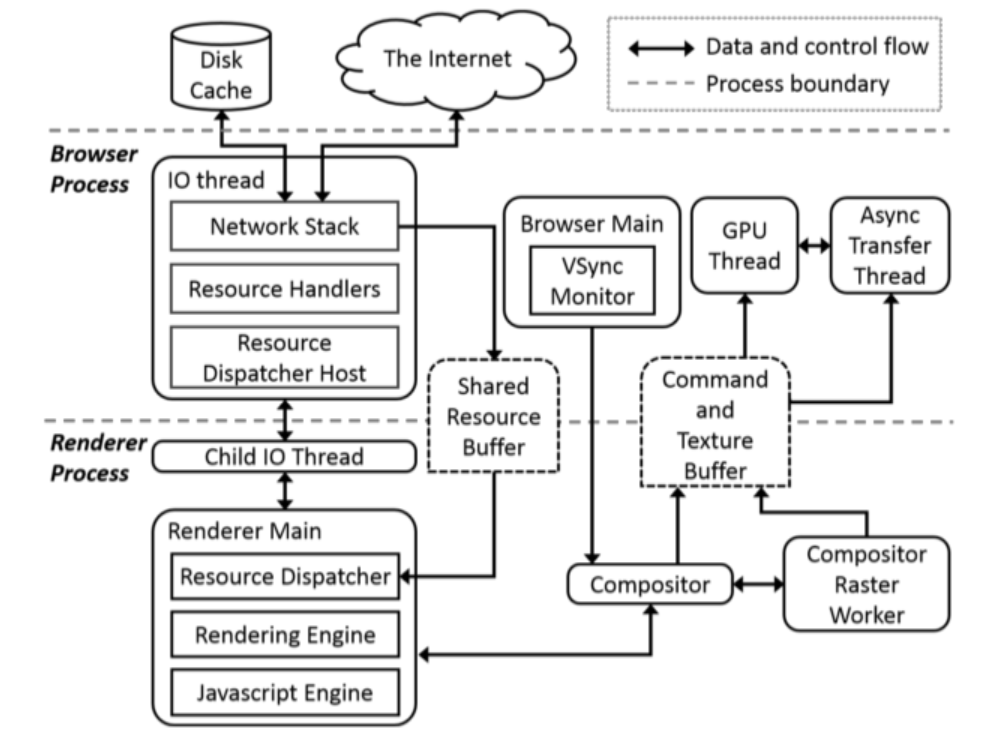
\includegraphics[width=3.4in]{./figure1}
	\caption{Chromium浏览器的体系结构}\label{fig:tasks}
\end{figure}

如图1所示, Chromium使用单个浏览器进程和多个Renderer进程的多进程体系结构。 每个Renderer进程运行一个渲染引擎的实例(以前是WebKit\cite{4},现在是Blink\cite{5})以及解析和执行Web内容的JavaScript引擎。 每个Renderer进程通常对应于Web浏览器UI中的一个选项卡。 浏览器进程运行网络堆栈并从网络中为所有呈现器进程获取网络资源,从而在所有呈现器进程之间共享高效的网络资源。 渲染器进程在沙盒环境中运行,对客户端设备和网络的访问受限,防止渲染引擎中的漏洞侵害整个Web浏览器。

Chromium中的每个进程都有多个线程,。进程和线程被设计为异步工作。浏览器进程和Renderer进程通过IPC机制(例如命名管道)相互通信,并使用共享内存交换数据。浏览器进程将获取的Web资源放入共享资源缓冲区,Renderer进程会从该缓冲区读取数据以创建相应网页的图形层。合成器线程然后将生成的图形数据保存到命令和纹理缓冲区中,以便在浏览器进程中进行GPU处理,因为沙盒渲染器进程没有直接访问GPU的权限。 GPU线程将最终屏幕图像生成到显示帧缓冲区中以显示在设备屏幕上。

图形组成和GPU处理由来自Android框架的称为垂直同步(VSync)的回调驱动。每个VSync信号指示显示帧的开始,以便在下一个VSync之前生成图形数据并将其移动到显示帧缓冲区以供在屏幕上绘制。垂直同步信号每秒产生60次。在浏览器进程中,浏览器主线程的VSync监视器监视VSync信号,并将它们转发到呈现器进程中的合成器线程。

图1所示的体系结构也适用于基于Chromium源代码构建的Google Chrome,Opera Mobile和Android stock 浏览器\cite{6}\cite{8}。浏览器共享相同的渲染引擎,JavaScript引擎和底层核心模块。

\subsection{Energy Cost Of Page Loading}

Web资源处理是浏览的主要组件之一,同时还有资源下载和内容渲染。 Web资源处理通常包括HTML和CSS解析,图像解码,Javascript执行以及更新DOM树和图形层。在Chromium中,只要呈现器进程通知了浏览器进程中可用的数据,就会执行上述处理。如图1所示,这两个进程使用共享资源缓冲区交换数据。浏览器进程在套接字处理程序上使用read系统调用来从网络接收网页资源。每个读取系统调用都会将接收到的数据直接写入资源缓冲区,默认情况下最大数据大小为32 KB。在每次读取系统调用时,无论接收到多少数据,浏览器进程都会立即通知呈现器进程开始处理接收到的数据。

尽管立即处理接收到的数据是很自然的,并且可以最大限度地减少页面加载时间,但这不是节能的。原因在于许多读取系统调用会返回少量数据,从而导致Browser进程和Renderer进程之间的大量IPC。平均而言,每个网页的IPC总数为871(每秒176)。每个IPC都有一个固定的开销。此外,网络资源处理中还有其他开销。每次处理数据块时,即使数据块很小,Renderer进程也必须经历整个数据渲染管道。特别是对于图像数据,Compositor,Raster Worker和Async Transfer线程中涉及许多图形活动。因此,累积的管理费用会浪费大量能源。

加载网页时,Chromium会逐步处理Web资源,并不断将部分渲染的显示结果更新到屏幕上。如图1所示,屏幕更新由VSync信号驱动。在接收到VSync信号后,合成器线程通过共享命令和纹理缓冲区将当前渲染图形数据传送到浏览器进程的GPU线程。 GPU线程然后在GPU上执行特定于平台的图形命令以将所有纹理合成为最终图形结果以显示在屏幕上。这种数据渲染和屏幕更新的图形管道称为内容绘制。

加载网页时可能会出现许多内容,但是在大多数情况下,内容绘制只会在屏幕上产生非常小的甚至不可见的变化。这些无法察觉或非常小的屏幕变化无助于改善用户体验。但是,它们会导致整个图形处理流水线和两个流程之间的IPC发生开销,从而导致不必要的能源成本。

除此以外,big.LITTLE的节能潜力并没有被充分利用。大多数情况下,线程都是在大内核上执行的,而小内核却处于空闲的状态。

导致这一现象的原因在于操作系统是基于负载驱动方法调度线程的,该方法偏好性能而不是节能。调度程序试图尽快完成一个线程,而不是节省更多的能量。在对称多核架构上,由于所有的CPU核心都是相同的,这种负载驱动的方法是节能的。如果一个线程可以更快完成任务,CPU可以更快地进入睡眠状态以节省能量。\cite{7}但是,在像big.LITTLE这样的异构多核架构中,尽早完成线程可能不会降低能源成本。与一个大内核相比,一个小内核执行每个指令的能耗更低。因此,在较小的内核上运行线程虽然需要更长的时间,但消耗的能量更少。因此,如果一个线程可以容忍延迟,就可以安排在一个小内核上运行。但是,操作系统无法知道线程可以承受多少延迟,因此无法决定是否在较小的内核上运行线程以提高能效。

\section{OVERVIEW}

在本节中,我们将介绍旨在更好地平衡移动网页加载中的能源成本和性能的几种技术。

\subsection{Network-AwareWeb Resource Processing}

进行网络资源处理的频率会影响浏览器的性能和能效。频繁的资源处理显然会导致能源效率低下和大量的能源消耗。但是对网络资源进行批处理可能会延迟Web资源的处理并增加页面加载时间。

为此,我们建议设计适应网络资源下载速度的网络资源处理,也就是$Network-aware\ Resource\ Processing$(NRP)\cite{1}。一个基本的基本原则是下载得越快,批量就应该越大。也就是说,当下载速度较慢时应该使用批量的规模变小,以免在Web资源处理中带来过多的延迟。我们强制浏览器进程缓冲从网络接收到的数据,并且只有在缓冲数据量大于阈值时才通知渲染器进程。这样,我们可以减少网络资源处理的次数以及涉及的IPC数量,从而可以降低能源成本。

为了平衡资源处理延迟和能源效率之间的平衡,我们设计缓冲区阈值$buf\_threshold$和总缓冲区大小$buf\_size$以适应资源下载速度$net\_goodput$,如下所示:

\begin{align*}
buf\_threshold &= \alpha * net\_goodput \\
buf\_size &= \beta * buf\_threshold
\end{align*}

其中$net\_goodput$是使用指数加权移动平均线(EWMA)估算的,这是一个基于线性历史的估计器,其平滑因子为$0.3$。\cite{9}\cite{10}参数$\alpha$表示一段数据在缓冲区中可以经历的最大等待时间,这个时间的设置需要我们在节能和资源处理延迟之间找到平衡。参数$\beta$控制总缓冲区大小。缓冲器过度使用时会增加,使用不足时会减少。

附加参数$buf\_size$旨在最大限度地减少总内存使用量。处理每个Web资源时,它需要分配一个大小为$buf\_size$的专用缓冲区。由于加载网页时可能会有很多网络资源,因此如果缓冲区大小很大,则总内存使用率可能较高。通过我们的方法,我们将$buf\_size$设计得很小,同时又足够大以允许下载跟上资源处理。

理想情况下,NRP应该直接适应屏幕上用户感知的内容更改。也就是说,缓冲应该适应Web内容在屏幕上显示的速度。然而,从接收到的数据中检测显示的内容的变化是困难的,并且由于像JavaScript这样的动态内容而造成很高的开销。因此,我们选择网络吞吐量(接收数据的速率)作为显示内容变化的间接但低开销的指标。通过根据吞吐量来控制缓冲器阈值,我们平衡能量成本和网络资源处理的延迟。

为了进一步减少NRP对页面加载时间的影响,我们不将缓冲应用于可能延迟其他资源下载的关键资源。这些关键资源包括主框架的顶层HTML资源(称为Chromium中的主要资源)以及网页的子框架或iframe。这些资源在从网络接收到后立即处理。此外,即使块大小小于$buf\_threshold$,我们也不会缓冲Web资源的最后一块,以防止小的最后一个数据块长时间停留在资源缓冲区中。这是通过检测响应是否完成来实现的,这由浏览器中的网络流解析器执行。因此,它也适用于动态内容。如果响应完成,我们通知Renderer进程立即开始处理所有收到的数据,而不是等待达到$buf\_threshold$。

\subsection{Adaptive Content Painting}

内容绘制需要在用户体验和能量开销之间进行权衡。尽管高帧速率可以提供非常流畅的用户体验,但它可能会导致GPU和CPU渲染网页时产生高昂的开销,并且与高分辨率结合时会消耗大量能量\cite{12}。。由于大多数内容渲染只会产生零或非常小的可见屏幕变化,所以多种内容渲染可以聚合在一起以节省能量而不损害用户体验。受此启发,我们将内容绘画设计为适应屏幕上的可见变化,我们将其称为$adaptive\ content\ painting$(ACP)\cite{1}。

我们引入了一个名为$paint\_rate$的新参数,该参数限制了内容绘制的速度并动态适应内容更改速度,因此我们可以聚合内容绘画以节省能量,同时保留用户体验。对于给定的$paint\_rate$值,ACP强制实际的内容绘制速率不会超过$paint\_rate$的值(实际速率可能低于$paint\_rate$)。 $paint\_rate$参数的范围从最小绘画率到最大绘画率。 $paint\_rate$的初始值被设置为最小值。当内容快速变化时,$paint\_rate$参数会增加,反之亦然。在合成器线程将更改后的内容绘制到屏幕上后,如果网页继续更改并需要更新屏幕以反映更改,我们将参数线性地增加1以达到最大值。另一方面,当合成器将所有更改传送到屏幕后,当网页显示内容停止改变时,我们将参数降低到最小值。

我们将最大绘制速率限制为10帧/秒以平衡能量成本和内容显示的平滑度。我们认为,10帧/秒应该足够平滑,因为1)在页面加载时,网页内容仅部分显示,因此对用户体验的影响很小(特别是在小屏幕智能手机上);和2)屏幕上的内容变化率通常很低。此外,现有的研究\cite{39}表明,延迟高达100毫秒通常是不可感知的。因此,我们认为10帧/秒(即每帧100毫秒)在用户体验和节能之间提供了良好的折衷。当内容变化缓慢时,我们将最小绘制速率设置为2帧/秒以节省更多能量。

理想情况下,ACP技术应量化画框之间的视觉变化以适应内容的变化程度。但是,这样做需要逐个像素比较连续的帧,这会造成大量计算并因此导致高能量成本。因此,我们使用线性增加$paint\_rate$参数的轻量级方法,而无需任何额外的计算成本。

此外,内容绘画应该意识到用户交互。用户触摸屏幕时应使用较高的渲染率,以确保用户体验顺畅。因此,在我们的实施中,我们还会在用户触摸屏幕时检测用户输入和停止速率限制。

NRP和ACP的两种技术并不完全独立。 NRP批量处理资源并因此减慢内容绘画。与NRP类似,ACP还减少了浏览器进程和渲染器进程之间的IPC数量,以节省能源。


\subsection{Application-Assisted Scheduling}

为了更好地利用big.LITTLE架构来节省能源,我们建议利用浏览器的内部知识进行节能高效的调度。我们允许浏览器决定一个线程是应该运行在一个大的还是小的核心上,而不是让OS任务调度程序通过被动地观察线程的负载来做出所有的调度决策。浏览器比OS调度器知道更多有关它们线程的信息,例如线程执行的是什么类型的任务,线程有多重要,线程可以容忍的结束时间,线程的语义以及它们之间的关系。因此,浏览器可能会更好地决定将线程分配给大内核还是小内核。我们称这种技术为$application-assisted\ scheduling$(AAS)\cite{1}。

我们设计适用于服务质量(QoS)的AAS技术,因为QoS对用户体验非常重要。 QoS通过浏览器的帧速率估算。 QoS要求根据$paint\_rate$的变化值进行动态调整。如果ACP不工作,则该要求被固定为涂漆速率的最大限制(即10帧/秒)。 AAS首先在小内核上分配与QoS有关的一组线程,并监视当前帧速率。当前帧速率落后于QoS要求时,AAS认为它是QoS的违规。例如,如果$paint\_rate$的值为5,则将QoS定义为在200 ms内绘制每个帧。如果浏览器无法在200 ms内绘制每帧,AAS会判定QoS已被违反,从而迁移大内核相关的线程。当当前帧速率以稳定的方式超过QoS要求时,AAS将这些线程带回到小内核。 AAS在发现当前帧速率与窗口上的QoS要求之间的累积差距不小于阈值时做出这样的决定。因此,在满足QoS的同时,其相应的线程保持在小核心上以节约能量而不损害用户体验。

为了更好地利用小核心来节省更多的能量,我们设计了AAS,以保守的方式将线程从小核心转移到大核心,使用三秒钟的时间窗口,并将线程从大核心移回到小核心核心使用更短的一秒钟时间窗口。

ACP调整$paint\_rate$限制,而AAS仅监视实际帧速率(帧绘制时间)并安排线程以满足限制。由于$paint\_rate$只设置最大涂装速率而不是固定涂装速率,因此AAS技术和帧速率之间没有严格的循环依赖关系。

AAS中的小内核和大内核之间的线程迁移对于所有应用程序都是通用的。 AAS技术动态地改变了QoS相关线程的亲和性,因此不需要将特定线程硬分配给核心。但是,应由AAS管理哪些线程以及如何定义QoS是特定于应用程序的。在第5节中,我们将向我们展示Chromium的哪些线程应用AAS技术。


\section{conclusion}

本文提出了多种有效的技术来优化智能手机网页加载的能耗。 其中两项技术,网络感知资源处理和自适应内容绘制,旨在解决当前移动Web浏览器在其内容处理和图形处理管道中的能源效率问题。 第三种是应用辅助调度,旨在平衡节能和QoS big.LITTLE平台之间的权衡。 这些技术被实施在了Chromium和Firefox中,并使用真实世界的网站和最新一代的智能手机进行了全面评估。 实验结果和用户研究表明,这些技术能够显着降低网页加载的能源成本,并引入难以察觉的页面加载时间增加。

\bibliographystyle{abbrv}
\begin{thebibliography}{1}
	\bibitem[1]{1}
	\bibsc{Bui D H, Liu Y, Kim H, et al}
	\newblock Rethinking energy-performance trade-off in mobile web page loading.
	\newblock \bibemphic{Proceedings of the 21st Annual International Conference on Mobile Computing and Networking. ACM, 2015: 14-26.}
	
	\bibitem[2]{2}
	\newblock ARM big.LITTLE technology.
	\newblock http://www.thinkbiglittle.com.
	
	\bibitem[3]{3}
	\newblock Alexa, Top Sites in United States.
	\newblock http://www.alexa.com/topsites/countries/US.
	
	\bibitem[4]{4}
	\newblock WebKit. \\
	\newblock http://www.webkit.org.
	
	\bibitem[5]{5}
	\newblock Blink. \\
	\newblock http://www.chromium.org/blink.
	
	\bibitem[6]{6}
	\newblock Differences between Google Chrome and Linux distro Chromium. \\
	\newblock http://code.google.com/p/chromium /wiki/ChromiumBrowserVsGoogleChrome.
	
	\bibitem[7]{7}
	\newblock A. Carroll and G. Heiser. Mobile multicores: Use them or waste them.
	\newblock \bibemphic{Proc. USENIX HotPower, 2013.}
	
	\bibitem[8]{8}
	\newblock A. Cunningham. New Opera for Android looks like Opera, tastes like Chrome.
	\newblock http://arstechnica.com/ information-technology/2013/05/new-opera-for- android-looks-like-opera-tastes-like-chrome.
	
	\bibitem[9]{9}
	\newblock Q. He, C. Dovrolis, and M. Ammar. On the predictability of large transfer TCP throughput.
	\newblock \bibemphic{Proc. ACMSIGCOMM, 2005.}
	
	\bibitem[10]{10}
	\newblock M. Mirza, J. Sommers, P. Barford, and Xiaojin Zhu. A machine learning approach to TCP throughput prediction.
	\newblock \bibemphic{Networking, IEEE/ACMTransactions on, 18(4):1026–1039, 2010.}
	
	\bibitem[12]{12}
	\newblock K. W. Nixon, X. Chen, H. Zhou, Y. Liu, and Y. Chen. Mobile gpu power consumption reduction via dynamic resolution and frame rate scaling.
	\newblock \bibemphic{HotPower, 2014.}
	
	\bibitem[13]{13}
	\newblock N. Thiagarajan, G. Aggarwal, A. Nicoara, D. Boneh, and J. P. Singh. Who Killed My Battery: Analyzing Mobile Browser Energy Consumption.
	\newblock \bibemphic{Proc. WWW, 2012.}
	
	\bibitem[14]{14}
	\newblock Y. Zhu and V. J. Reddi. High-performance and Energy-efficient Mobile Web Browsing on Big/Little Systems.
	\newblock \bibemphic{Proc. IEEE HPCA, 2013.}
	
	\bibitem[15]{15}
	\newblock M. Butkiewicz, H. V. Madhyastha, and V. Sekar. Understanding Website Complexity: Measurements, Metrics, and Implications.
	\newblock \bibemphic{Proc. ACM IMC, 2011.}
	
	\bibitem[16]{16}
	\newblock M. Dong and L. Zhong. Chameleon: A Color-adaptive Web Browser for Mobile OLED Displays.
	\newblock \bibemphic{Proc. ACM MobiSys, 2011.}
	
	\bibitem[17]{17}
	\newblock M. Dong and L. Zhong. Chameleon: A Color-Adaptive Web Browser for Mobile OLED Displays.
	\newblock \bibemphic{IEEE Transactions on Mobile Computing (TMC), 2012.}
	
	\bibitem[18]{18}
	\newblock F. Qian, S. Sen, and O. Spatscheck. Characterizing Resource Usage for Mobile Web Browsing.
	\newblock \bibemphic{Proc. ACM MobiSys, 2014.}
	
	\bibitem[19]{19}
	\newblock B. Zhao, Q. Zheng, G. Cao, and S. Addepalli. Energy-Aware Web Browsing in 3G Based Smartphones.
	\newblock \bibemphic{Proc. IEEE ICDCS, 2013.}
	
	\bibitem[20]{20}
	\newblock SPDY. \\
	\newblock http://www.chromium.org/spdy.
	
	\bibitem[21]{21}
	\newblock Hypertext transfer protocol version 2.0, draft-ietf-httpbis-http2-07.
	\newblock http://tools.ietf.org/ html/draft-ietf-httpbis-http2-07.
	
	\bibitem[22]{22}
	\newblock X. S. Wang, A. Balasubramanian, A. Krishnamurthy, and D. Wetherall. How Speedy is SPDY?
	\newblock \bibemphic{Proc. USENIX NSDI, 2014.}
	
	\bibitem[23]{23}
	\newblock Z. Wang, F. X. Lin, L. Zhong, and M. Chishtie. How Far Can Client-only Solutions Go for Mobile Browser Speed?
	\newblock \bibemphic{Proc. USENIX NSDI, 2014.}
	
	\bibitem[24]{24}
	\newblock Y. Ma, X. Liu, S. Zhang, R. Xiang, Y. Liu, and T. Xie. Measurement and Analysis of Mobile Web Cache Performance.
	\newblock \bibemphic{Proc. WWW, 2015.}
	
	\bibitem[25]{25}
	\newblock L. A. Meyerovich and R. Bodik. Fast and parallel webpage layout.
	\newblock \bibemphic{Proc. WWW, 2010.}
	
	\bibitem[26]{26}
	\newblock A. Pathak, Y. C. Hu, and M. Zhang. Where is the Energy Spent Inside My App?: Fine Grained Energy Accounting on Smartphones with Eprof.
	\newblock \bibemphic{Proc. ACM EuroSys, 2012.}
	
	\bibitem[27]{27}
	\newblock F. Xu, Y. Liu, T. Moscibroda, R. Chandra, L. Jin, Y. Zhang, and Q. Li. Optimizing Background Email Sync on Smartphones.
	\newblock \bibemphic{Proc. ACM MobiSys, 2013.}
	
	\bibitem[28]{28}
	\newblock A. Carroll and G. Heiser. Unifying DVFS and offlining in mobile multicores.
	\newblock \bibemphic{Proc. IEEE RTAS, 2014.}
	
\end{thebibliography}


\end{document}
